\section{PASS Discrimination}
    The use of squeezed states instead of coherent states allows us to overcome the limits
    of precedent systems. The representation of a noisy squeezed state is given in 
    \ref{squeezedStates}. This section initially discusses the advantages of using squeezed states 
    without photon addition; then it evaluates the effect of the photon addition
    in quantum OOK and BPSK systems.

    \subsection{Squeezed states discrimination}
        At first, we assess the effect of squeezing on the performance in absence of photon 
        addition and thermal noise. As for PACS systems, it can be useful to define the mean 
        number of photon $n_p$ in a squeezed state, which is given by
        \begin{equation}
            n_p(\mu,r) = \absolutevalue{\mu}^2 + \left(\sinh{r}\right)^2;
        \end{equation}
        where $\mu$ is the amplitude of the starter coherent state and the squeezing factor
        is $\zeta = r e^{i\theta}$. The minimum value of $n_p$ is given by $n_p(0,r) = \sinh{r}^2$.

        \begin{figure}[ht]
            \begin{center}
                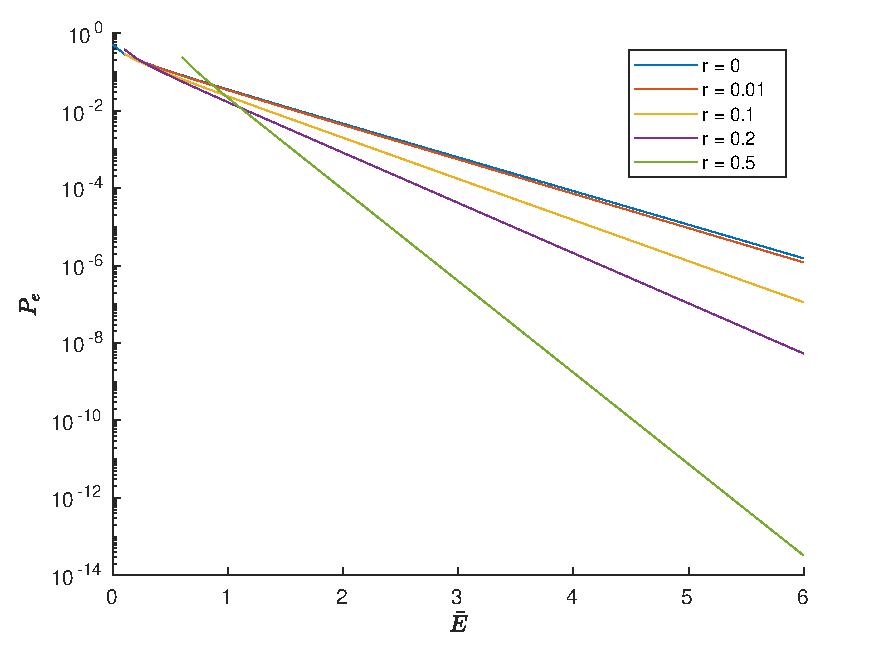
\includegraphics[width=0.75\textwidth]{fig3.5.pdf}
                \caption{MDEP of squeezed state BPSK system. 
                    $N=30$, $\bar{n}=0$, $\theta=\pi$, $p_0=p_1=1/2$}
                \label{fig:3.5}
            \end{center}     
        \end{figure}
        For a quantum squeezed states BPSK system, the MDEP, obtained with the Helstrom bound 
        \ref{eq:HelstromBound}, is plotted in figure \ref{fig:3.5} in function of $\bar{E}$,
        i.e the mean energy of the system (given by the sum of $n_p$ for each state), with:
        $\theta=\pi$, $N=30$, equiprobable symbols and $\bar{n}=0$.

        It can be noticed that the optimal configuration of $r$ depends on the energy in the 
        system. For low energy levels the squeezing has not a positive effect.

    \subsection{PASS discrimination}
        We are analyzing now the performance of a noisy photon added squeezed state system (PASS)
        \ref{PAS}, in OOK and BPSK configuration. The MDEP is found again with the Helstrom bound
        \ref{eq:HelstromBound}.
        As for the other systems, it is useful to define the mean number of photons $n_p$ for noisy 
        photon added squeezed states, that is given by:
        \begin{equation}
            n_p(\mu,\zeta,\bar{n}) = \frac{N_{k+1}(\mu,\zeta,\bar{n})}{N_k(\mu,\zeta,\bar{n})}-1,
            \label{eq:np_PASS}
        \end{equation}
        where
        \begin{equation}
            \begin{split}
                N_k(\mu,\zeta,\bar{n}) &= tr\{(\pmb{A}^\dagger)^k \pmb{\Xi}_{th}(\mu,\zeta) \pmb{A}^k\}\\
                                       &= tr\{(\pmb{A}^\dagger)^k \pmb{D}_\mu \pmb{S}_\zeta \pmb{\Xi}_{th}
                                        \pmb{S}_\zeta^\dagger \pmb{D}_\mu^\dagger \pmb{A}^k\}.
            \end{split}
        \end{equation}

        \paragraph{OOK PASS system}\mbox{}\\
        The constellation of a quantum OOK system with noisy PASS, is given by:
        \begin{equation}
            \begin{split}
                \pmb{\Xi}_0 &= \pmb{\Xi}_{th}^{(0)}(0,0)\\
                \pmb{\Xi}_1 &= \pmb{\Xi}_{th}^{(k)}(\mu,\zeta).
            \end{split}
        \end{equation}
        \begin{figure}[ht]
            \begin{center}
                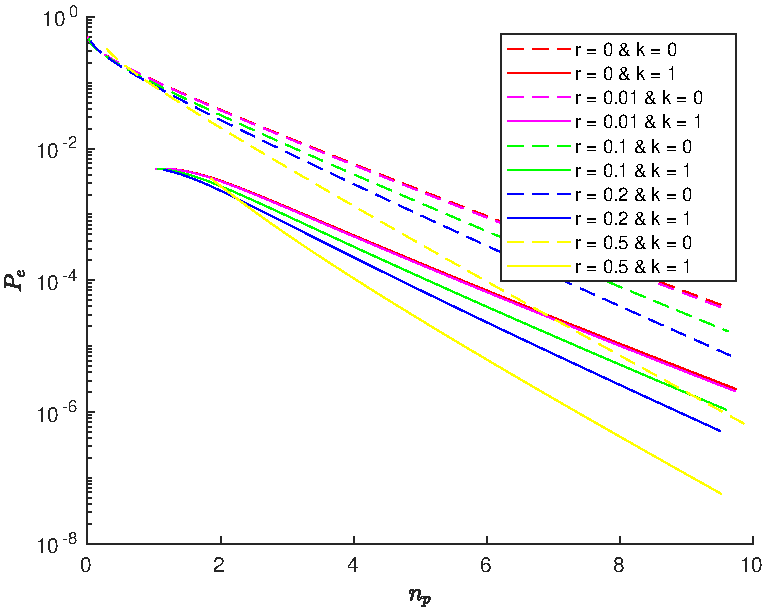
\includegraphics[width=0.75\textwidth]{fig3.6.pdf}
                \caption{MDEP of noisy PASS quantum OOK system.\\
                $N=30$, $\bar{n}=10^{-2}$, $\theta=\pi$ and $p_0=p_1=1/2$.}
                \label{fig:3.6}
            \end{center}
        \end{figure}
        In figure \ref{fig:3.6}, the MDEP of a quantum OOK noisy PASS system is plotted in function
        of the mean number of photon $n_p$ in the PASS (that is equivalent to the mean energy
        in the system). For the simulation are used $N=30$, $\bar{n}=10^{-2}$, $\theta=\pi$ and
        equiprobable symbols.
        It can be noticed that the photon addition significantly improves the performance of the system,
        at least for the plotted energy level.

        \paragraph{BPSK PASS system}\mbox{}\\
        Similary to the PACS BPSK, the constellation of PASS BPSK is given by:
        \begin{equation}
            \begin{split}
                \pmb{\Xi}_0 &= \pmb{\Xi}_{th}^{(k)}(-\mu,\zeta)\\
                \pmb{\Xi}_1 &= \pmb{\Xi}_{th}^{(k)}(\mu,\zeta).
            \end{split}
        \end{equation}
        \begin{figure}[ht]
            \begin{center}
                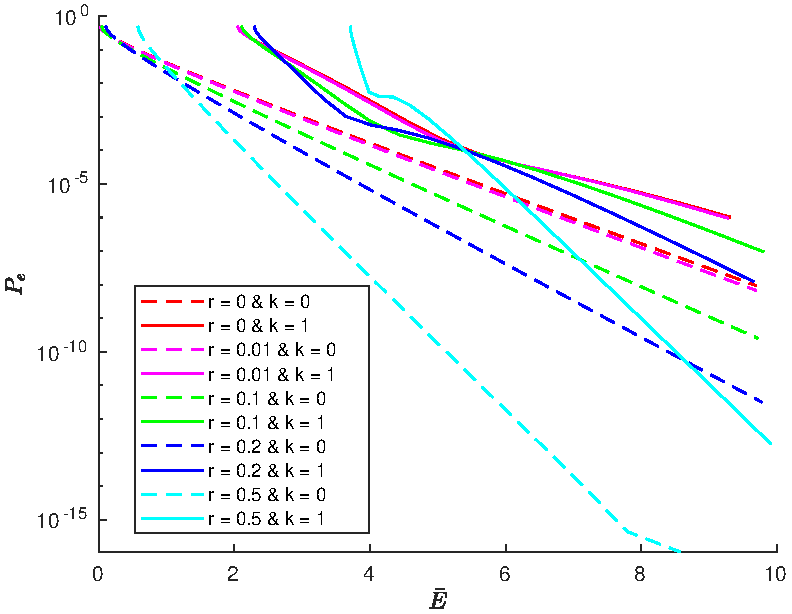
\includegraphics[width=0.75\textwidth]{fig3.7.pdf}
                \caption{MDEP of noisy PASS quantum BPSK system.\\
                $N=30$, $\bar{n}=10^{-2}$, $\theta=\pi$ and $p_0=p_1=1/2$.}
                \label{fig:3.7}
            \end{center}
        \end{figure}
        The figure \ref{fig:3.7} shows the effects of the photon addition in a quantum BPSK
        system, in terms of the mean energy in the system $\bar{E}$, given by the sum of 
        the mean photon number $n_p$ of $\pmb{\Xi}_0$ and $\pmb{\Xi}_1$. The parameters used
        for the simulation are $N=30$, $\bar{n}=10^{-2}$, $\theta=\pi$ and equiprobable symbols.
        As in PACS case, it is evident that the photon addition, in a BPSK system, has not
        the positive effect that has in an OOK system.